\section{Grasping}

\begin{frame}
\frametitle{Gripper \& Forward Kinematics}
\begin{columns}
\column{0.5\textwidth}
\begin{center}
\begin{figure}[!htb]
\centering
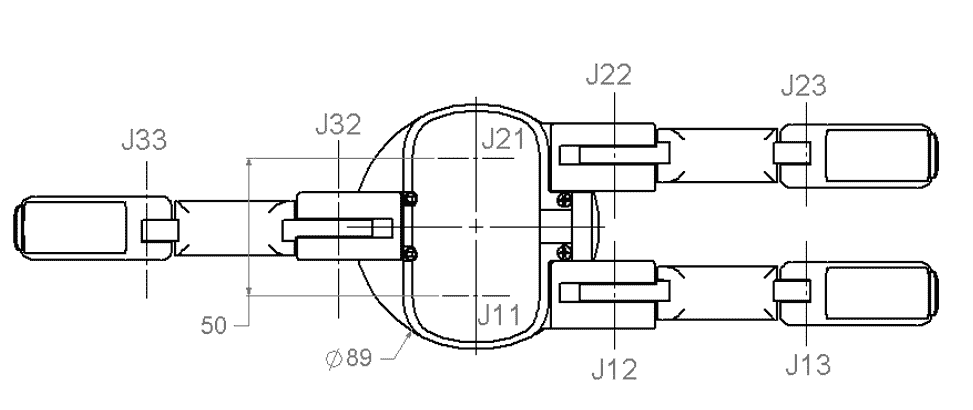
\includegraphics[width=\textwidth]{../images/bh8-282-top-only.png}\\
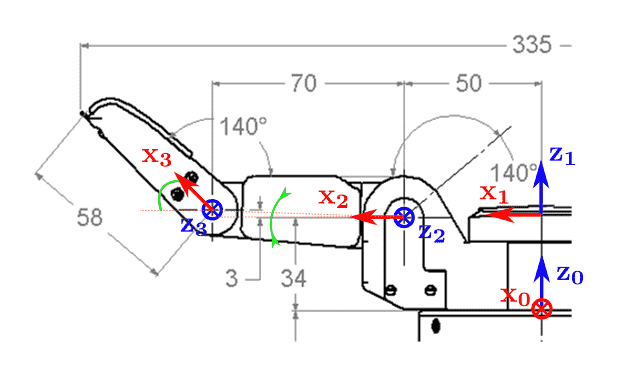
\includegraphics[width=\textwidth]{../images/bh8-282-generalized-finger-fwd-kin.png}\\
\end{figure}
\end{center}

\column{0.5\textwidth}
\resizebox*{\textwidth}{!}{
\begin{tabular}{ |c|c|c|c|c| } 
\hline
i & $θ_i$ (rad) & $L_{i-1}$ (m) & $d_i$ (m) & $α_{i-1}$ (rad) \\
\hline
1 (J11) & $θ_{11} - π/2$ & 0.025 & 0.0034 & 0 \\
2 (J12) & $θ_{12} + 0.04$ & 0.05 & 0 & $π/2$ \\
3 (J13) & $θ_{13} + 0.69$ & 0.07 & 0 & 0 \\
\hline
\end{tabular}
}
\vfill
\resizebox*{\textwidth}{!}{
\begin{tabular}{ |c|c|c|c|c| } 
\hline
i & $θ_i$ (rad) & $L_{i-1}$ (m) & $d_i$ (m) & $α_{i-1}$ (rad) \\
\hline
1 (J21) & $θ_{21} - π/2$ & 0.025 & 0.0034 & 0 \\
2 (J22) & $θ_{22} + 0.04$ & 0.05 & 0 & $π/2$ \\
3 (J23) & $θ_{23} + 0.69$ & 0.07 & 0 & 0 \\
\hline
\end{tabular}
}
\vfill
\resizebox*{\textwidth}{!}{
\begin{tabular}{ |c|c|c|c|c| } 
\hline
i & $θ_i$ (rad) & $L_{i-1}$ (m) & $d_i$ (m) & $α_{i-1}$ (rad) \\
\hline
1 & $π/2$ & 0 & 0.0034 & 0 \\
2 (J32) & $θ_{32} + 0.04$ & 0.05 & 0 & $π/2$ \\
3 (J33) & $θ_{33} + 0.69$ & 0.07 & 0 & 0 \\
\hline
\end{tabular}
}
\end{columns}
\end{frame}


\begin{frame}
\frametitle{Gripper Inverse Kinematics}
Standard solutions of a RRR kinematic chain, using the law of cosines
\begin{columns}
\column{0.5\textwidth}
\begin{center}
\begin{figure}[!htb]
\centering
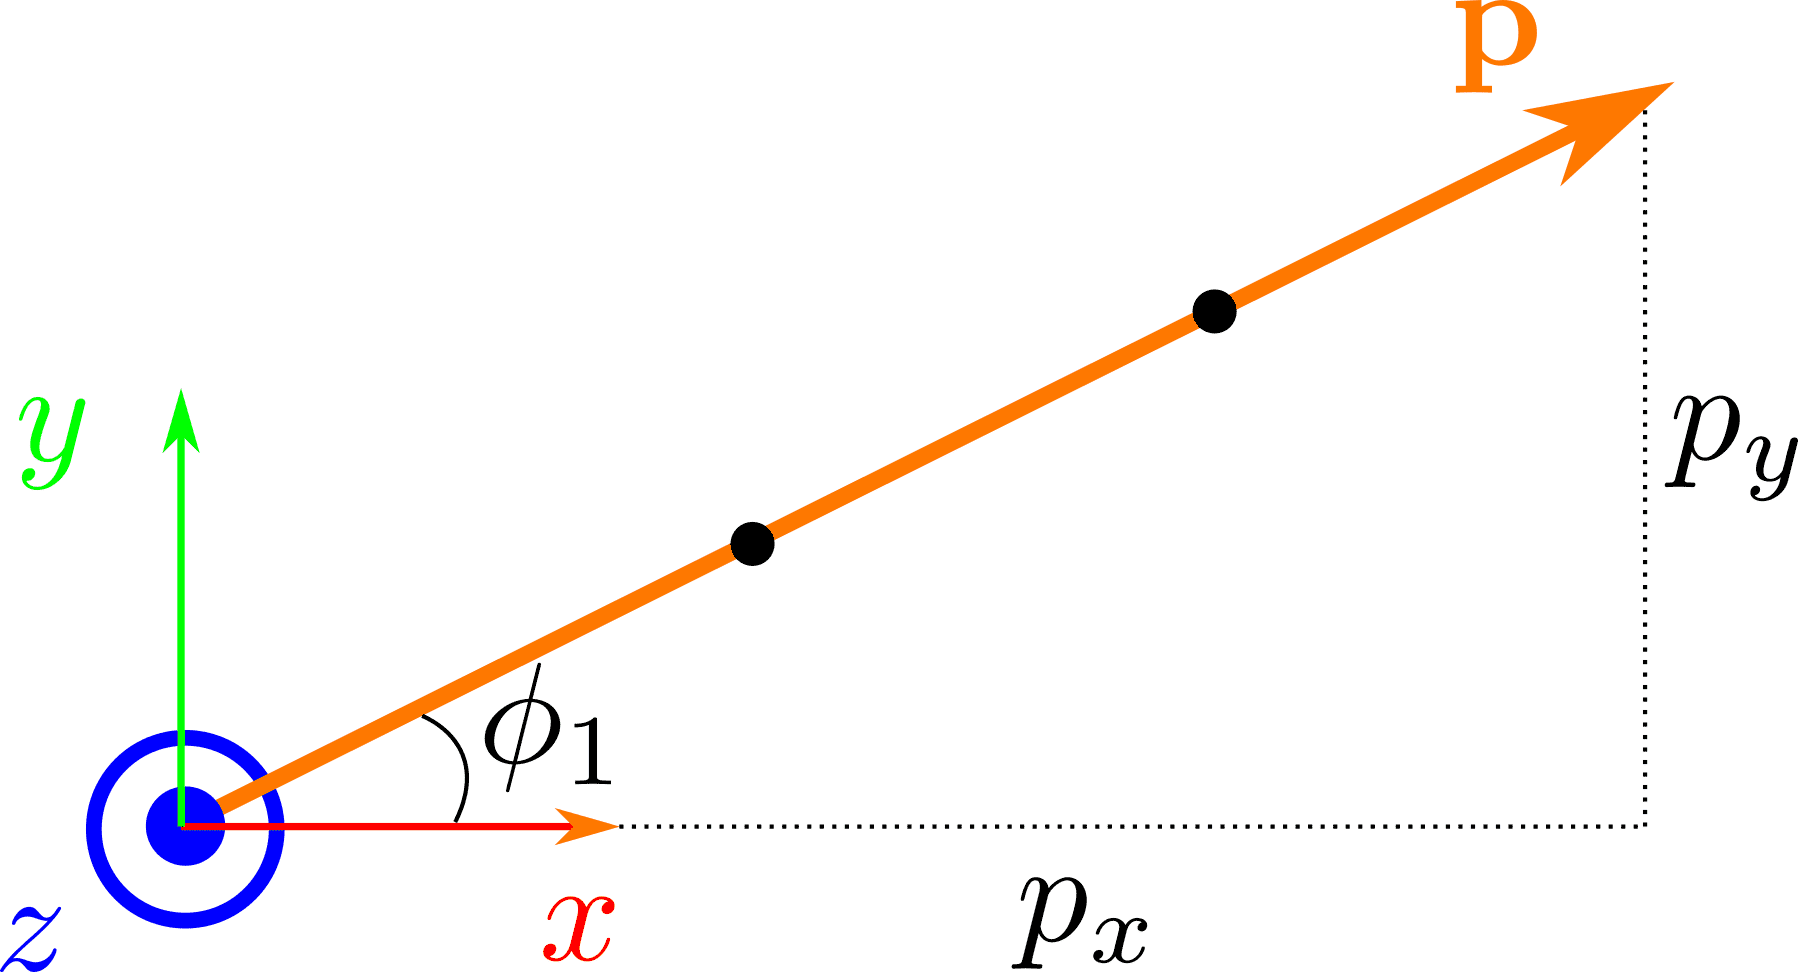
\includegraphics[width=0.8\textwidth]{../images/grasper-rrr-top.png}\\
\caption{top view}
\end{figure}
\end{center}
\column{0.5\textwidth}
\begin{center}
\begin{figure}[!htb]
\centering
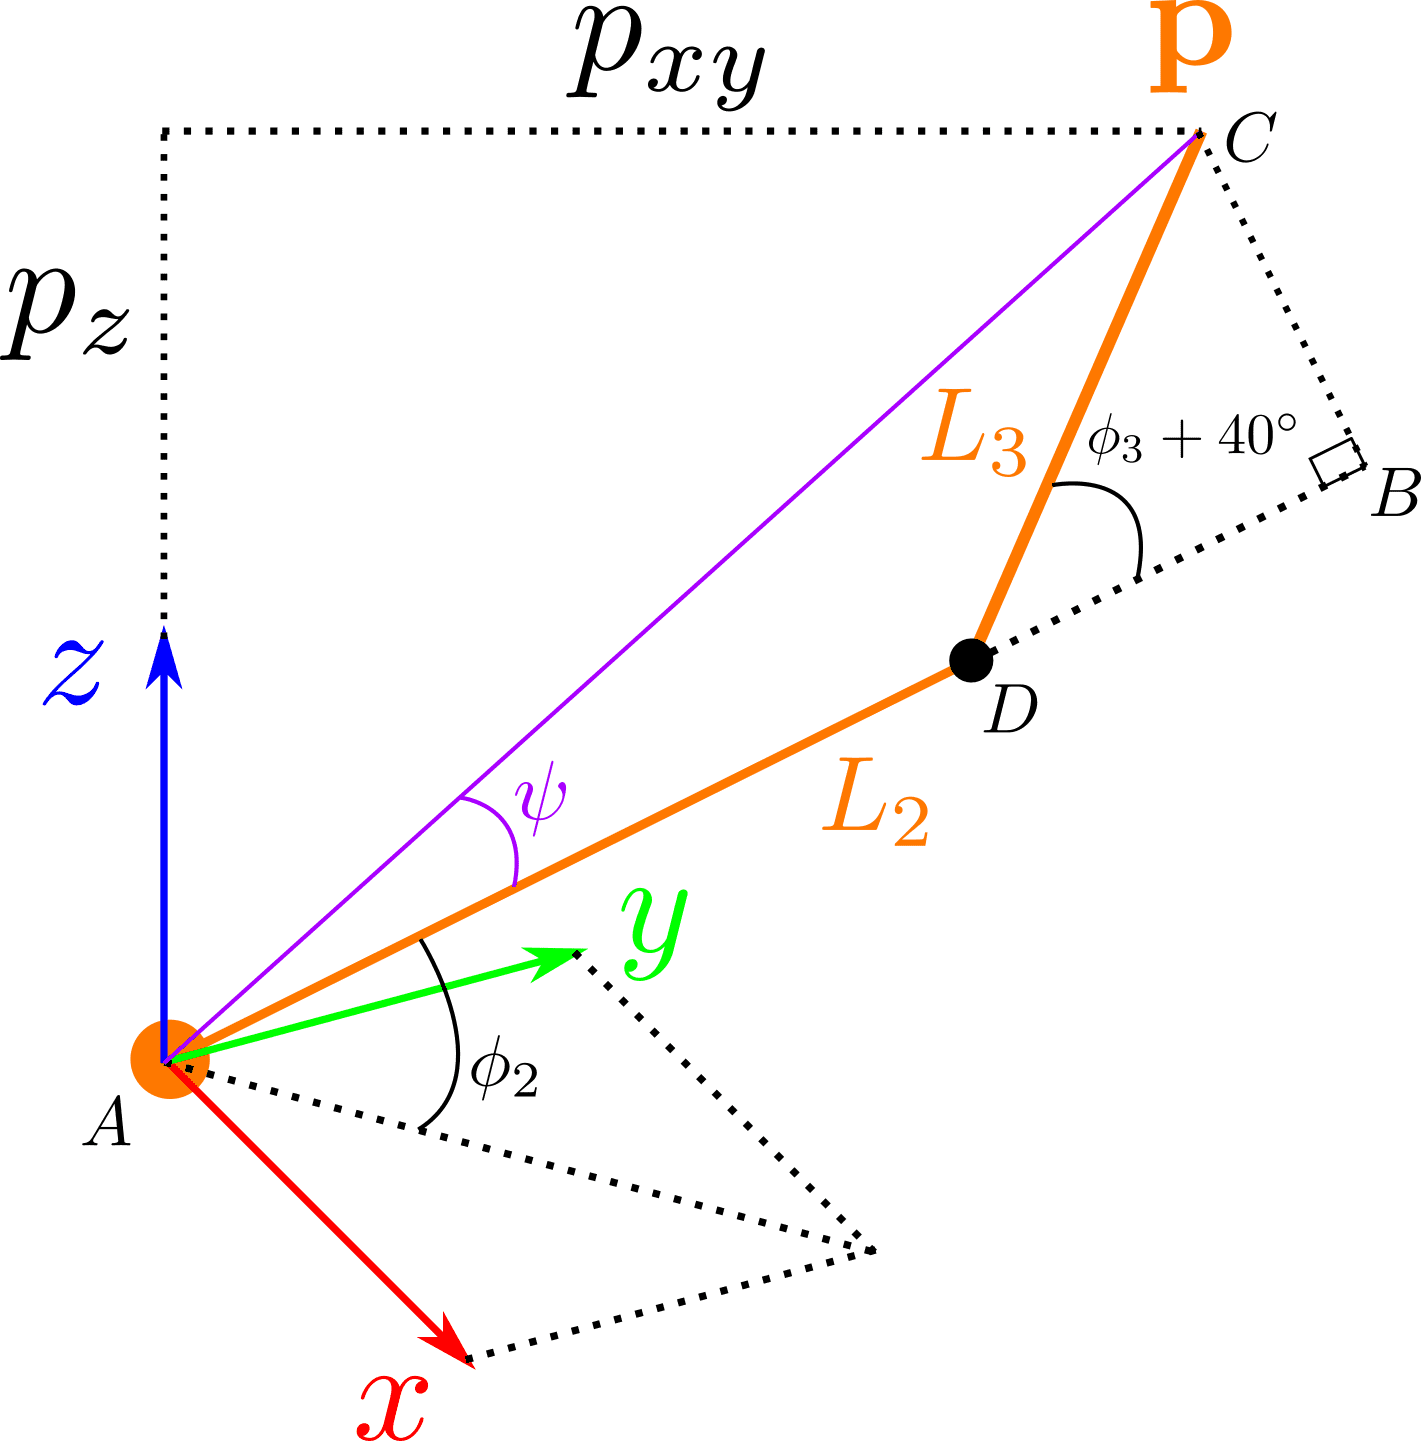
\includegraphics[width=0.8\textwidth]{../images/grasper-rrr-side.png}\\
\caption{side view}
\end{figure}
\end{center}
\end{columns}
\end{frame}
